\chapter{정합 실험 기록}
\label{ch:experiments}

크롭한 점군(target)과 source 점군의 정합 실험을 누적 기록한다. 각 행은
\begin{lstlisting}
scripts/reg-bench.py <source> <target> --label <name> [--gpu]
\end{lstlisting}
한 번의 실행으로 추가되며, 원본 데이터는
\ccfile{experiments/registration-results.csv}, 아래 표는 그로부터 자동
생성된다 (이 파일은 손으로 수정하지 않는다).

\textbf{지표 정의} --- 모든 알고리즘에 동일하게 적용되는 공통 지표다
(\ccfile{backend/registration}의 \texttt{alignmentMetric}):
\begin{itemize}
  \item \textbf{rmse} --- 추정 변환을 적용한 \emph{후}, source 각 점에서
  target 최근접점까지 거리의 RMS. 작을수록 좋고, 대략 점 간격/노이즈
  수준이면 성공.
  \item \textbf{inliers} --- 그 거리가 target 점 간격의 $3$배 미만인 source
  점 수. source 크기에 가까울수록 좋다 (부분 중첩이면 중첩 영역 크기 수준).
  \item \textbf{conf.} --- (gradient-SDF + 불확실성 채널 한정) 최종 포즈에서
  $\chi^2$-정규화 잔차 $u_i=r_i^2/\sigma^2(\mathbf{x}_i)$ 를 필드의 확신
  영역($\sigma^2<\tfrac{1}{2}\sigma_f^2$)에서 평가했을 때 $u_i<4$ 인 비율.
  포즈가 맞으면 $\approx 1$, ``그럴듯하게 틀린'' 정합이면 낮다. `-' = 미지원.
  \item \textbf{conv.} --- 백엔드의 자체 수렴 판정 ($\circ$/$\times$;
  \textbf{err}는 실행 실패).
  \item \textbf{time} --- 정합 1회의 벽시계 시간 (공통 지표 계산 포함).
\end{itemize}

% AUTO-GENERATED by scripts/reg-bench.py - do not edit by hand.
% Source of truth: experiments/registration-results.csv
\begin{longtable}{p{0.24\linewidth}p{0.13\linewidth}llrrrr}
\toprule
\textbf{case (source $\to$ target)} & \textbf{algo} & \textbf{conv.} & \textbf{rmse} & \textbf{inliers} & \textbf{conf.} & \textbf{time(s)} & \textbf{date} \\
\midrule
bag:hesai $\to$ crop & gicp & $\times$ & 2.74574 & 10212 & - & 17.62 & 2026-06-11 15:28 \\
bag:hesai $\to$ crop & icp & $\times$ & 2.70646 & 3284 & - & 19.05 & 2026-06-11 15:28 \\
bag:hesai $\to$ crop & icp-plane & $\times$ & 2.72664 & 4440 & - & 15.11 & 2026-06-11 15:28 \\
bag:hesai $\to$ crop & kiss & $\times$ & 2.67776 & 4 & - & 12.09 & 2026-06-11 15:28 \\
bag:hesai $\to$ crop & kiss-gicp & $\times$ & 2.65279 & 2004 & - & 22.92 & 2026-06-11 15:28 \\
bag:hesai $\to$ crop & vgicp & $\times$ & 2.75794 & 7408 & - & 12.92 & 2026-06-11 15:28 \\
bag:hap100 $\to$ crop & gicp & $\times$ & 5.31451 & 5253 & - & 79.52 & 2026-06-11 15:31 \\
bag:hap100 $\to$ crop & icp & $\circ$ & 5.11101 & 0 & - & 112.87 & 2026-06-11 15:31 \\
bag:hap100 $\to$ crop & icp-plane & $\circ$ & 4.97018 & 5253 & - & 60.59 & 2026-06-11 15:31 \\
bag:hap100 $\to$ crop & kiss & $\times$ & 4.09824 & 1494 & - & 37.42 & 2026-06-11 15:31 \\
bag:hap100 $\to$ crop & kiss-gicp & $\times$ & 4.13849 & 2228 & - & 37.23 & 2026-06-11 15:31 \\
bag:hap100 $\to$ crop & vgicp & $\circ$ & 5.10775 & 0 & - & 112.63 & 2026-06-11 15:31 \\
bag:hap101 $\to$ crop & gicp & $\circ$ & 3.95147 & 0 & - & 46.72 & 2026-06-11 15:42 \\
bag:hap101 $\to$ crop & icp & $\circ$ & 3.95147 & 0 & - & 48.85 & 2026-06-11 15:42 \\
bag:hap101 $\to$ crop & icp-plane & $\circ$ & 3.95147 & 0 & - & 44.27 & 2026-06-11 15:42 \\
bag:hap101 $\to$ crop & kiss & $\circ$ & 3.03093 & 10598 & - & 21.96 & 2026-06-11 15:42 \\
bag:hap101 $\to$ crop & kiss-gicp & $\circ$ & 3.03052 & 10598 & - & 21.63 & 2026-06-11 15:42 \\
bag:hap101 $\to$ crop & vgicp & $\circ$ & 3.95147 & 0 & - & 46.73 & 2026-06-11 15:42 \\
bag:hesai $\to$ crop & gsdf-gpu & $\circ$ & 3.16037 & 304 & 0.005 & 144.87 & 2026-06-11 17:26 \\
bag:hap100 $\to$ crop & gsdf-gpu & $\circ$ & 3.96163 & 276 & 0.034 & 162.40 & 2026-06-11 17:28 \\
bag:hap101 $\to$ crop & gsdf-gpu & $\circ$ & 3.02596 & 7018 & 1.000 & 58.07 & 2026-06-11 17:31 \\
hap101-f0\_\_crop & bufferx & $\circ$ & 3.03073 & 10593 & - & 26.78 & 2026-06-16 15:51 \\
hap101-f0\_\_crop & bufferx-gicp & $\circ$ & 3.03048 & 10598 & - & 27.10 & 2026-06-16 15:51 \\
hap101-f0\_\_crop & gsdf-gpu & $\circ$ & 3.01394 & 752 & 0.029 & 65.13 & 2026-06-16 15:51 \\
hap101-f0\_\_crop & g3reg & $\circ$ & 3.03125 & 10596 & - & 30.76 & 2026-06-16 20:34 \\
hap101-f0\_\_crop & g3reg-gicp & $\circ$ & 3.03049 & 10598 & - & 30.89 & 2026-06-16 20:34 \\
\bottomrule
\end{longtable}


\section{정합 결과 시각화}
각 백엔드의 정렬 결과를 3D로 겹쳐 본 그림이다 (\ccfile{scripts/reg-figures.py} 로 자동 생성).
% AUTO-GENERATED by scripts/reg-figures.py - do not edit by hand.
% One overlay figure per registration case (aligned source over target).
\begin{figure}[htbp]
  \centering
  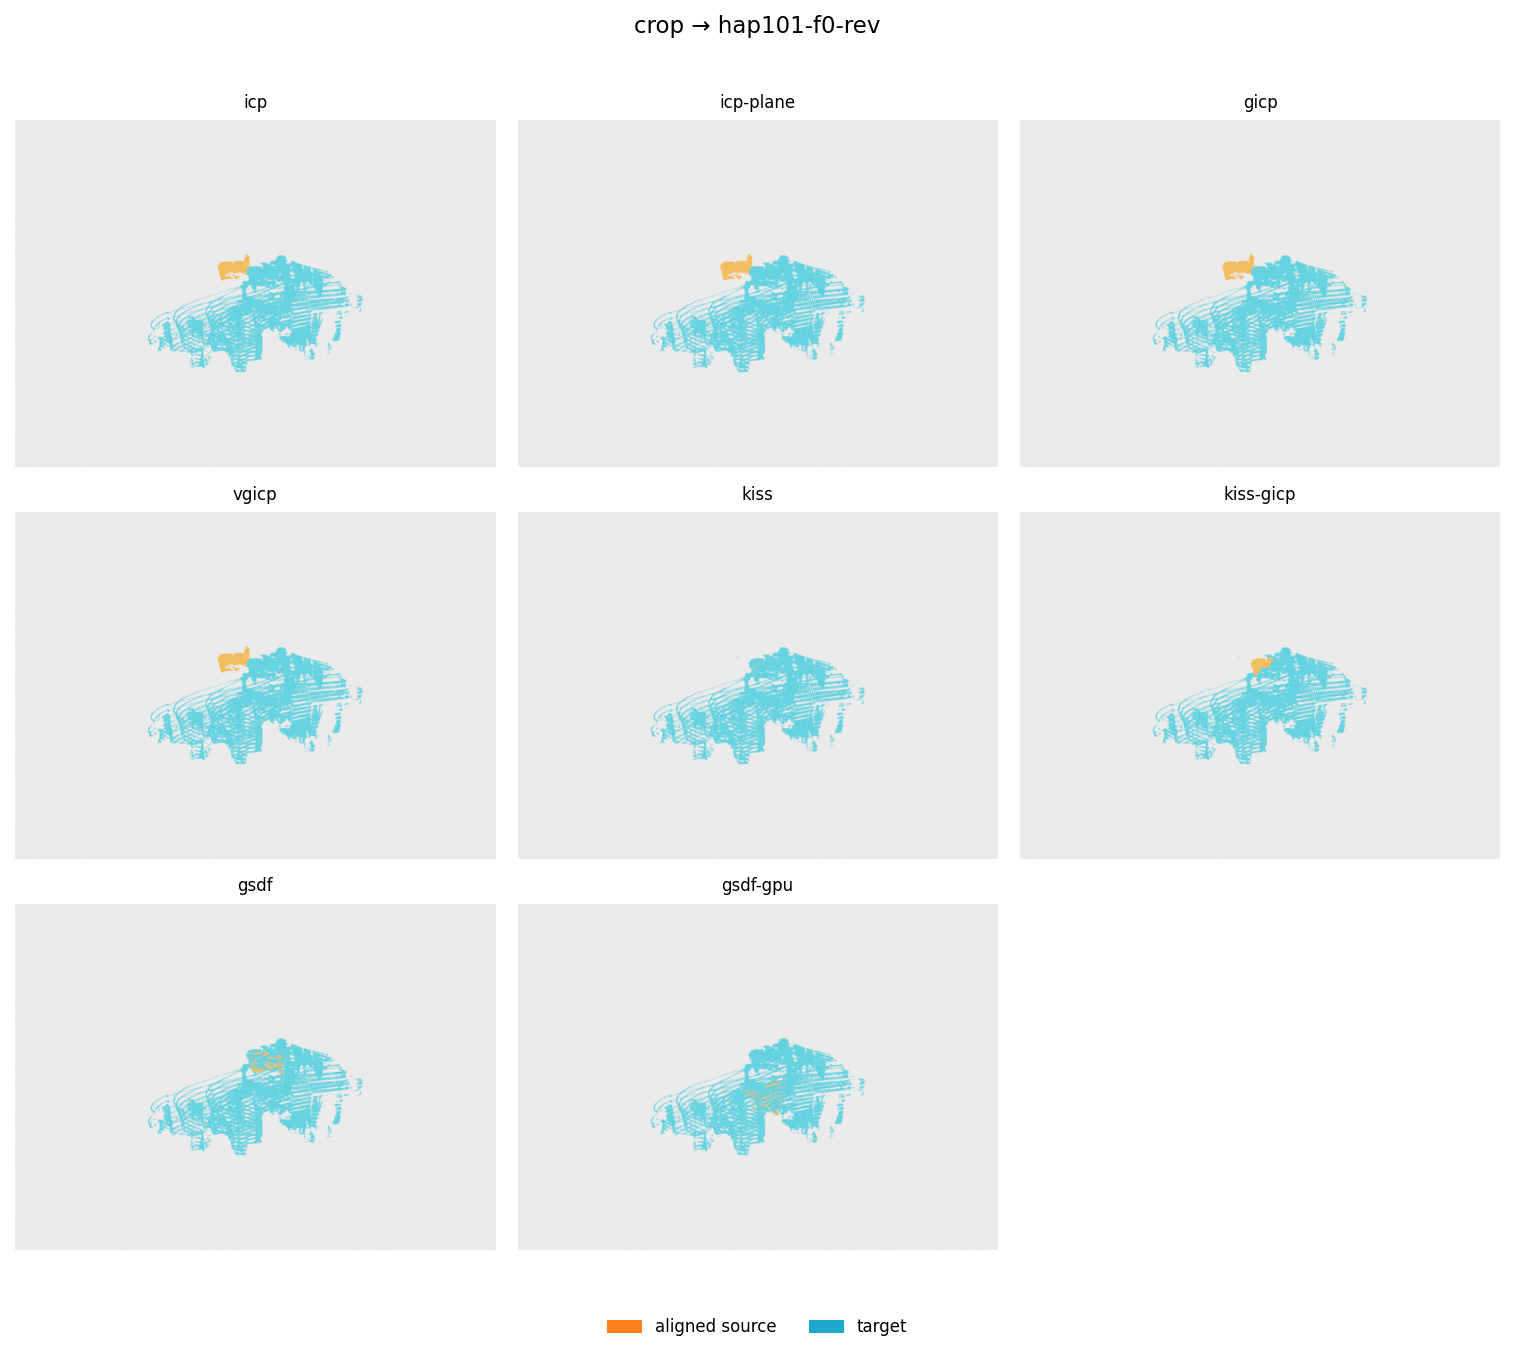
\includegraphics[width=\linewidth]{figures/crop__hap101-f0-rev_overlay.png}
  \caption{정합 결과 3D 오버레이: crop\_\_hap101-f0-rev (주황 = 정렬된 source, 청록 = target).}
  \label{fig:overlay-crop__hap101-f0-rev}
\end{figure}

\begin{figure}[htbp]
  \centering
  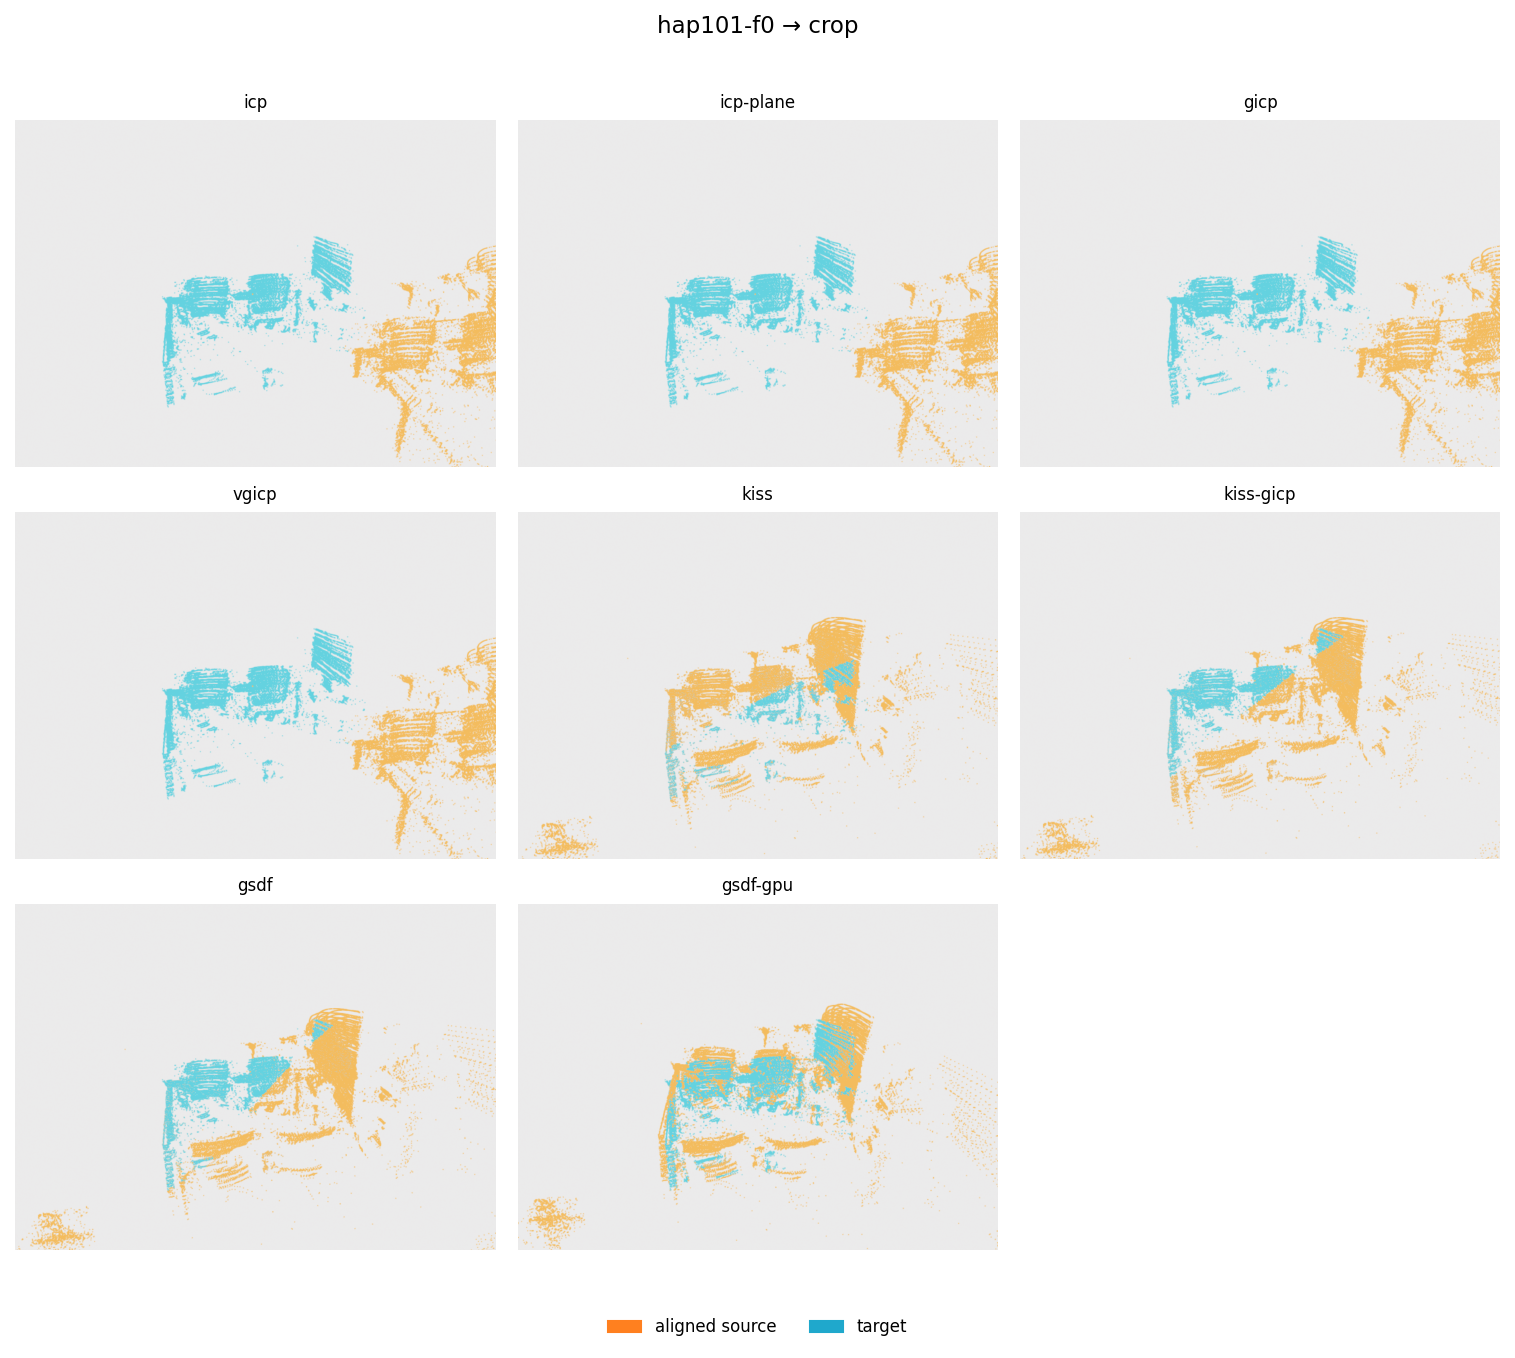
\includegraphics[width=\linewidth]{figures/hap101-f0__crop_overlay.png}
  \caption{정합 결과 3D 오버레이: hap101-f0\_\_crop (주황 = 정렬된 source, 청록 = target).}
  \label{fig:overlay-hap101-f0__crop}
\end{figure}

